\documentclass[border={0.000000bp 0.000000bp 0.000000bp 0.000000bp}, 11pt]{standalone}
\pdfinfoomitdate=1
\pdftrailerid{}
\pdfsuppressptexinfo=1
\pdfinfo{ /Creator () /Producer () }

\usepackage{tikz}
\usepackage{xcolor}
\usetikzlibrary{shapes.misc}
\usetikzlibrary{backgrounds}

\definecolor{dotColorA}{HTML}{000000}
\definecolor{dotColorB}{HTML}{000000}
\definecolor{dotColorC}{HTML}{000000}
\definecolor{dotColorD}{HTML}{000000}
\definecolor{dotColorE}{HTML}{000000}
\definecolor{dotColorF}{HTML}{000000}
\definecolor{dotColorG}{HTML}{000000}
\definecolor{dotColorH}{HTML}{000000}
\definecolor{dotColorI}{HTML}{000000}
\definecolor{dotColorJ}{HTML}{000000}
\definecolor{dotColorK}{HTML}{000000}
\definecolor{dotColorL}{HTML}{000000}

\definecolor{labelBgColorA}{HTML}{FFFFFF}
\definecolor{labelBgColorB}{HTML}{FFFFFF}
\definecolor{labelBgColorC}{HTML}{FFFFFF}
\definecolor{labelBgColorD}{HTML}{FFFFFF}
\definecolor{labelBgColorE}{HTML}{FFFFFF}
\definecolor{labelBgColorF}{HTML}{FFFFFF}
\definecolor{labelBgColorG}{HTML}{FFFFFF}
\definecolor{labelBgColorH}{HTML}{FFFFFF}
\definecolor{labelBgColorI}{HTML}{FFFFFF}
\definecolor{labelBgColorJ}{HTML}{FFFFFF}
\definecolor{labelBgColorK}{HTML}{FFFFFF}
\definecolor{labelBgColorL}{HTML}{FFFFFF}

\definecolor{labelTextColorA}{HTML}{000000}
\definecolor{labelTextColorB}{HTML}{000000}
\definecolor{labelTextColorC}{HTML}{000000}
\definecolor{labelTextColorD}{HTML}{000000}
\definecolor{labelTextColorE}{HTML}{000000}
\definecolor{labelTextColorF}{HTML}{000000}
\definecolor{labelTextColorG}{HTML}{000000}
\definecolor{labelTextColorH}{HTML}{000000}
\definecolor{labelTextColorI}{HTML}{000000}
\definecolor{labelTextColorJ}{HTML}{000000}
\definecolor{labelTextColorK}{HTML}{000000}
\definecolor{labelTextColorL}{HTML}{000000}

\definecolor{linkColorA}{HTML}{000000}
\definecolor{linkColorB}{HTML}{000000}
\definecolor{linkColorC}{HTML}{000000}
\definecolor{linkColorD}{HTML}{000000}
\definecolor{linkColorE}{HTML}{000000}
\definecolor{linkColorF}{HTML}{000000}
\definecolor{linkColorG}{HTML}{000000}
\definecolor{linkColorH}{HTML}{000000}
\definecolor{linkColorI}{HTML}{000000}
\definecolor{linkColorJ}{HTML}{000000}
\definecolor{linkColorK}{HTML}{000000}
\definecolor{linkColorL}{HTML}{000000}

\def\textA{\textsc{amoc}}
\def\textB{\textsc{binseg}}
\def\textC{\textsc{bocpd}}
\def\textD{\textsc{bocpdms}}
\def\textE{\textsc{cpnp}}
\def\textF{\textsc{ecp}}
\def\textG{\textsc{kcpa}}
\def\textH{\textsc{pelt}}
\def\textI{\textsc{prophet}}
\def\textJ{\textsc{rfpop}}
\def\textK{\textsc{segneigh}}
\def\textL{\textsc{wbs}}

\begin{document}
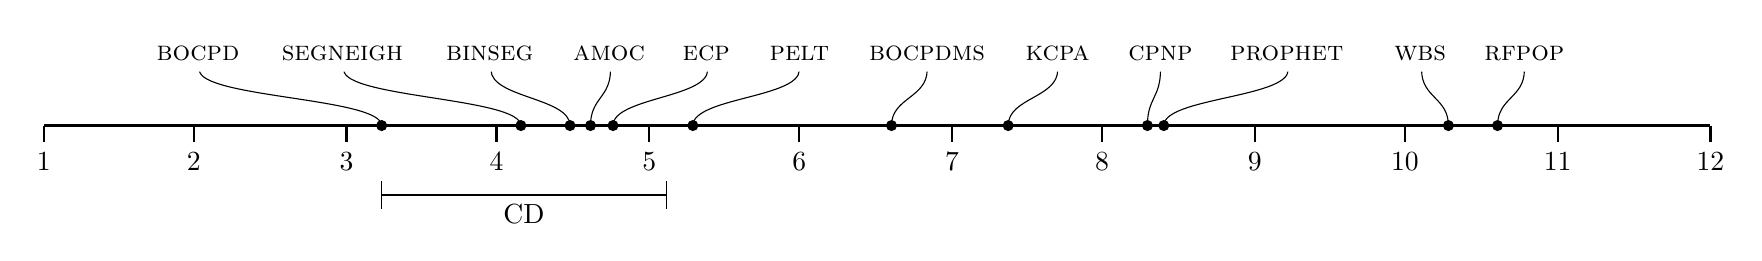
\begin{tikzpicture}[x=1bp,y=-1bp]

% shift for the margin
\begin{scope}[shift={(0, 0)}]
% main layer
\begin{scope}[shift={(0, 75)}]
% axis
\begin{scope}
\draw[very thick] (0, 0) -- (600, 0);
\end{scope}

% axis layer
\begin{scope}
\begin{scope}[shift={(0, 0)}]
\draw[thick] (0, 0) -- (0, -6pt)
node[anchor=north] {1};
\end{scope}
\begin{scope}[shift={(54, 0)}]
\draw[thick] (0, 0) -- (0, -6pt)
node[anchor=north] {2};
\end{scope}
\begin{scope}[shift={(109, 0)}]
\draw[thick] (0, 0) -- (0, -6pt)
node[anchor=north] {3};
\end{scope}
\begin{scope}[shift={(163, 0)}]
\draw[thick] (0, 0) -- (0, -6pt)
node[anchor=north] {4};
\end{scope}
\begin{scope}[shift={(218, 0)}]
\draw[thick] (0, 0) -- (0, -6pt)
node[anchor=north] {5};
\end{scope}
\begin{scope}[shift={(272, 0)}]
\draw[thick] (0, 0) -- (0, -6pt)
node[anchor=north] {6};
\end{scope}
\begin{scope}[shift={(327, 0)}]
\draw[thick] (0, 0) -- (0, -6pt)
node[anchor=north] {7};
\end{scope}
\begin{scope}[shift={(381, 0)}]
\draw[thick] (0, 0) -- (0, -6pt)
node[anchor=north] {8};
\end{scope}
\begin{scope}[shift={(436, 0)}]
\draw[thick] (0, 0) -- (0, -6pt)
node[anchor=north] {9};
\end{scope}
\begin{scope}[shift={(490, 0)}]
\draw[thick] (0, 0) -- (0, -6pt)
node[anchor=north] {10};
\end{scope}
\begin{scope}[shift={(545, 0)}]
\draw[thick] (0, 0) -- (0, -6pt)
node[anchor=north] {11};
\end{scope}
\begin{scope}[shift={(600, 0)}]
\draw[thick] (0, 0) -- (0, -6pt)
node[anchor=north] {12};
\end{scope}
\end{scope}

% link layer
\begin{scope}
\draw[color=linkColorA, thin] (196.8058968058968, 0) .. controls
(196.8058968058968, -10.0) and (204.0, -10.0) .. (204.0, -20.0);
\draw[color=linkColorB, thin] (189.4348894348894, 0) .. controls
(189.4348894348894, -10.0) and (161.0, -10.0) .. (161.0, -20.0);
\draw[color=linkColorC, thin] (121.62162162162163, 0) .. controls
(121.62162162162163, -10.0) and (56.0, -10.0) .. (56.0, -20.0);
\draw[color=linkColorD, thin] (305.1597051597052, 0) .. controls
(305.1597051597052, -10.0) and (318.0, -10.0) .. (318.0, -20.0);
\draw[color=linkColorE, thin] (397.2972972972973, 0) .. controls
(397.2972972972973, -10.0) and (402.0, -10.0) .. (402.0, -20.0);
\draw[color=linkColorF, thin] (204.91400491400495, 0) .. controls
(204.91400491400495, -10.0) and (239.0, -10.0) .. (239.0, -20.0);
\draw[color=linkColorG, thin] (347.17444717444715, 0) .. controls
(347.17444717444715, -10.0) and (365.0, -10.0) .. (365.0, -20.0);
\draw[color=linkColorH, thin] (233.66093366093367, 0) .. controls
(233.66093366093367, -10.0) and (272.0, -10.0) .. (272.0, -20.0);
\draw[color=linkColorI, thin] (403.1941031941032, 0) .. controls
(403.1941031941032, -10.0) and (448.0, -10.0) .. (448.0, -20.0);
\draw[color=linkColorJ, thin] (523.3415233415234, 0) .. controls
(523.3415233415234, -10.0) and (533.0, -10.0) .. (533.0, -20.0);
\draw[color=linkColorK, thin] (171.74447174447172, 0) .. controls
(171.74447174447172, -10.0) and (108.0, -10.0) .. (108.0, -20.0);
\draw[color=linkColorL, thin] (505.6511056511057, 0) .. controls
(505.6511056511057, -10.0) and (496.0, -10.0) .. (496.0, -20.0);
\end{scope}

% label layer
\begin{scope}
\begin{scope}[shift={(185, -34)}]
\fill[color=labelBgColorA, rounded corners=2pt]
(0, 0) rectangle (37, 14.62708) node[midway, yshift=-.75bp, anchor=center, text=labelTextColorA] {\strut \textA};
\end{scope}
\begin{scope}[shift={(139, -34)}]
\fill[color=labelBgColorB, rounded corners=2pt]
(0, 0) rectangle (43, 14.62708) node[midway, yshift=-.75bp, anchor=center, text=labelTextColorB] {\strut \textB};
\end{scope}
\begin{scope}[shift={(35, -34)}]
\fill[color=labelBgColorC, rounded corners=2pt]
(0, 0) rectangle (41, 14.62708) node[midway, yshift=-.75bp, anchor=center, text=labelTextColorC] {\strut \textC};
\end{scope}
\begin{scope}[shift={(291, -34)}]
\fill[color=labelBgColorD, rounded corners=2pt]
(0, 0) rectangle (54, 14.62708) node[midway, yshift=-.75bp, anchor=center, text=labelTextColorD] {\strut \textD};
\end{scope}
\begin{scope}[shift={(385, -34)}]
\fill[color=labelBgColorE, rounded corners=2pt]
(0, 0) rectangle (34, 14.62708) node[midway, yshift=-.75bp, anchor=center, text=labelTextColorE] {\strut \textE};
\end{scope}
\begin{scope}[shift={(225, -34)}]
\fill[color=labelBgColorF, rounded corners=2pt]
(0, 0) rectangle (27, 14.62708) node[midway, yshift=-.75bp, anchor=center, text=labelTextColorF] {\strut \textF};
\end{scope}
\begin{scope}[shift={(348, -34)}]
\fill[color=labelBgColorG, rounded corners=2pt]
(0, 0) rectangle (34, 14.62708) node[midway, yshift=-.75bp, anchor=center, text=labelTextColorG] {\strut \textG};
\end{scope}
\begin{scope}[shift={(256, -34)}]
\fill[color=labelBgColorH, rounded corners=2pt]
(0, 0) rectangle (32, 14.62708) node[midway, yshift=-.75bp, anchor=center, text=labelTextColorH] {\strut \textH};
\end{scope}
\begin{scope}[shift={(421, -34)}]
\fill[color=labelBgColorI, rounded corners=2pt]
(0, 0) rectangle (53, 14.62708) node[midway, yshift=-.75bp, anchor=center, text=labelTextColorI] {\strut \textI};
\end{scope}
\begin{scope}[shift={(513, -34)}]
\fill[color=labelBgColorJ, rounded corners=2pt]
(0, 0) rectangle (40, 14.62708) node[midway, yshift=-.75bp, anchor=center, text=labelTextColorJ] {\strut \textJ};
\end{scope}
\begin{scope}[shift={(79, -34)}]
\fill[color=labelBgColorK, rounded corners=2pt]
(0, 0) rectangle (57, 14.62708) node[midway, yshift=-.75bp, anchor=center, text=labelTextColorK] {\strut \textK};
\end{scope}
\begin{scope}[shift={(481, -34)}]
\fill[color=labelBgColorL, rounded corners=2pt]
(0, 0) rectangle (29, 14.62708) node[midway, yshift=-.75bp, anchor=center, text=labelTextColorL] {\strut \textL};
\end{scope}
\end{scope}

% dots
\begin{scope}
\draw node [circle, inner sep=0pt, minimum size=4bp, 
fill=dotColorA] at (196.805897, 0) {};
\draw node [circle, inner sep=0pt, minimum size=4bp, 
fill=dotColorB] at (189.434889, 0) {};
\draw node [circle, inner sep=0pt, minimum size=4bp, 
fill=dotColorC] at (121.621622, 0) {};
\draw node [circle, inner sep=0pt, minimum size=4bp, 
fill=dotColorD] at (305.159705, 0) {};
\draw node [circle, inner sep=0pt, minimum size=4bp, 
fill=dotColorE] at (397.297297, 0) {};
\draw node [circle, inner sep=0pt, minimum size=4bp, 
fill=dotColorF] at (204.914005, 0) {};
\draw node [circle, inner sep=0pt, minimum size=4bp, 
fill=dotColorG] at (347.174447, 0) {};
\draw node [circle, inner sep=0pt, minimum size=4bp, 
fill=dotColorH] at (233.660934, 0) {};
\draw node [circle, inner sep=0pt, minimum size=4bp, 
fill=dotColorI] at (403.194103, 0) {};
\draw node [circle, inner sep=0pt, minimum size=4bp, 
fill=dotColorJ] at (523.341523, 0) {};
\draw node [circle, inner sep=0pt, minimum size=4bp, 
fill=dotColorK] at (171.744472, 0) {};
\draw node [circle, inner sep=0pt, minimum size=4bp, 
fill=dotColorL] at (505.651106, 0) {};
\end{scope}

% Critical difference
\def\posBest{121.6216216216216282}
\def\posCD{224.1075579550507086}
\begin{scope}
\draw (\posBest, 30) -- (\posBest, 20);
\draw (\posBest, 25) --node[below] {CD} (\posCD, 25);
\draw (\posCD, 30) -- (\posCD, 20);
\end{scope}

\end{scope}
\end{scope}
\end{tikzpicture}
\end{document}